\subsection{Column generation based primal heuristics}
\label{diving}

The BnP algorithm provides very good dual bounds. A good primal heuristic is needed for the algorithm to be efficient. As mentioned in \ref{heuristic-tree}, several heuristics based on the MIRUP property of the BPP and on rounding strategies are implemented. They are efficient but more sophisticated heuristics could have been implemented. Such heuristics are diving heuristics that are particularly well suited for BnP algorithms. The idea is to explore in a "smart" way an enumeration tree to get good feasible solutions fast. They can be combined with the BnP algorithm in two ways.

The first option is to create a new enumeration tree at each node aiming to get a good feasible solution. For a given node, we consider the optimal solution of \eqref{RMBPP} which can be fractional. Starting from this solution, an enumeration tree is explored in the same way as for the BnP algorithm but the branches are directly created using the variables $\alpha^p$ instead of an item pair $(i,j)$. At each node of this new enumeration tree, the most fractional $\alpha^p$ is fixed to $1$ in the up branch and to $0$ in the down branch and the master problem is re-optimized with the new constraint. The difference with the BRUSUC procedure is that new columns are generated to get better solutions.

The second option is to change completely the way branches are created in the BnP algorithm and to branch on the $\alpha^p$. In this case, the whole BnP correspond to the heuristic. However, branching constraints created with the $\alpha^p$ are weaker. In this case, we only have one enumeration tree but it can be deeper as dual bounds are worst.

In \cite{sadykov2013bin}, it is proposed to create a tabu list of the columns in order to diversify the search. The tabu list of columns at a branch-and-price node is the union of the tabu list of its ancestors and the columns chosen in previous child nodes of the ancestor. To get some feasible solutions faster, it is possible to use a maximum depth and a maximum discrepancy parameters in order to only explore a part of the enumeration tree. It can be very long to fully explore the tree and a good, but not necessary optimal, solution can be found using these two parameters.


\begin{figure}[!ht]
	\centering
	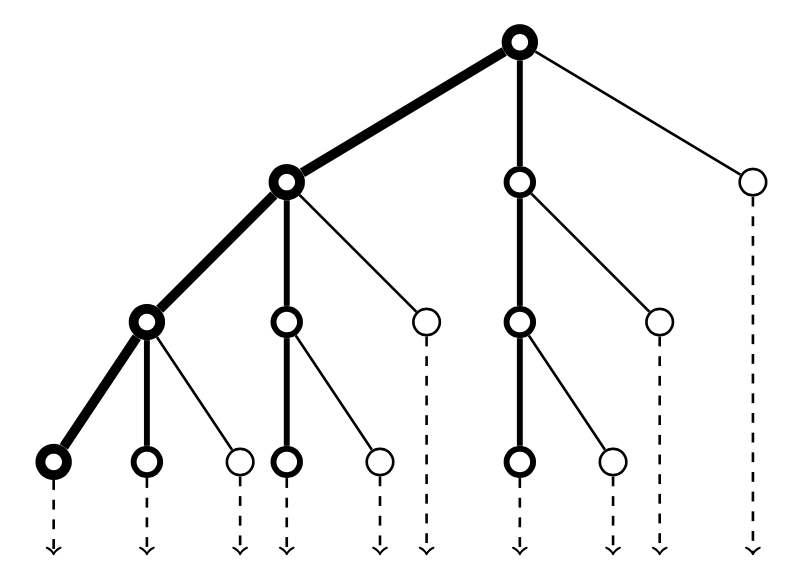
\includegraphics[width=0.4\linewidth]{img/diving.png}
	\caption{The enumeration tree of a diving heuristic with parameters maximum depth equal to 3 and maximum discrepancy equal to 2. The dotted lines are pure diving into the enumeration tree.}
\end{figure}